\hypertarget{hedendaagse-protheses}{%
\section{Hedendaagse protheses}\label{hedendaagse-protheses}}

Een prothese is een kunstmatige vervanging van een of meerdere
beschadigde of missende ledematen. Er bestaan verschillende soorten
protheses, van simpele nabootsingen van het desbetreffende ledemaat tot
volledig robotisch aangedreven protheses. Voor organen bestaan er ook
protheses, dit worden meestal implantaten genoemd, omdat de prothese
helemaal is weggewerkt in het lichaam. Een aantal verschillende
protheses zullen hier besproken worden, om een indruk te wekken van het
belang van protheses in de zorg.

\hypertarget{soorten-protheses}{%
\subsection{Soorten Protheses}\label{soorten-protheses}}

Je hebt veel verschillende soorten protheses, bijvoorbeeld een
beenprothese, borstprothese, armprothese, oogprothese, voetprothese en
handprothese. Ook zijn er hele bekende protheses, die in de volksmond
geen protheses meer worden genoemd. Denk aan een gehoorprothese
(gehoorapparaatje), een oogprothese (bril of lenzen) en tandprotheses
(kunstgebit). Elk van de eerdergenoemde protheses heeft een ander doel
en worden dus ook op een andere manier gemaakt, en meestal ook met
andere materialen.

\hypertarget{beenprothese}{%
\subsubsection*{Beenprothese}\label{beenprothese}}
\addcontentsline{toc}{subsubsection}{Beenprothese}

In de categorie beenprotheses bestaan er ook verschillende protheses, zo
is er een voetprothese, een onderbeenprothese met eventueel een
vervangende enkel, een bovenbeenprothese met een vervangende knie en
enkel en een totale beenprothese. Bij een amputatie onder de knie wordt
een onderbeenprothese het meeste toegepast. De onderbeenprothese bestaat
uit een koker die de stomp (waar de amputatie is verricht) nauwsluitend
omvat. De koker staat weer in verbinding met een prothesevoet, met
eventuele adapters. Er zijn veel verschillende soorten prothesevoeten,
hele simpele prothesevoeten, van simpel materiaal, tot prothesevoeten
van veerkrachtig materiaal die de energie van een stap opslaan om die te
gebruiken als je je weer afzet voor krachtigere stappen. Ook bestaan er
volledige mechanische beenprotheses, werkend met meerdere
microcontrollers. Een totale beenprothese wordt pas aangeraden als er
een totale beenamputatie heeft ondervonden. Het principe is hetzelfde
als hierboven is beschreven bij de onderbeenprotheses, alleen is er nu
nog een extra koker, voor het bovenbeen en een knie. De kunstknie heeft
een belangrijke taak, namelijk voorkomen dat de kokers onbedoeld kunnen
buigen en de gebruiker omvalt. Er zijn hiervoor speciale kunstknieën
ontworpen met een hydraulische of pneumatische vertraging, bij hele
geavanceerde knieën wordt het bijna elk aspect van een stap elektronisch
geregeld.

\hypertarget{implantaat}{%
\subsubsection*{Implantaat}\label{implantaat}}
\addcontentsline{toc}{subsubsection}{Implantaat}

Een implantaat is een prothese die helemaal is weggewerkt in het lichaam
(``Implantaat'' z.d.). Enkele voorbeelden hiervan zijn een hart-, heup-
en knie-implantaat. Ook zijn er bijvoorbeeld elektrische implantaten,
zoals pacemakers of een implanteerbare cardioverter-defibrillator. De
cardioverter-defibrillator kan een elektrische schok geven aan het hart
als het een ritmestoornis heeft. Dit zijn enkele voorbeelden van
implantaten.

\hypertarget{armprothese}{%
\subsubsection*{Armprothese}\label{armprothese}}
\addcontentsline{toc}{subsubsection}{Armprothese}

Ook bij armprotheses bestaan er verschillende soorten protheses. Van
vingerprotheses tot volledige arm protheses. De meest gebruikte techniek
om een armprothese te laten passen is om nadat de stomp een stabiel
volume heeft gekregen er een gipsafdruk van te maken. Daaraan wordt er
een stompkous gemaakt die om de stomp heen past en die men vast kan
maken aan de prothese (``Armprothese'' z.d.). Een van de vereiste van
een prothese is dat deze bruikbaar is in het dagelijks leven. Dit houdt
in dat men er voorwerpen mee kan vastpakken, vasthouden, een vinger op
kan steken en dergelijke acties. Dit moet aangestuurd worden. Er zijn
verschillende manieren om dit te doen, bijvoorbeeld door het gebruik van
de torso. Door deze in bepaalde richtingen te bewegen, trek je via een
harnas de connectie strak en beweegt de hand , dit mechanisme is
omschreven in Weir en Sensinger (2004). De `Body-powered Prosthesis' is
ook geïllustreerd in \xrefname{Fig.}\cref{fig:harnas}, waar het harnas
en de connectie met de hand te zien is.

\begin{figure}
\centering
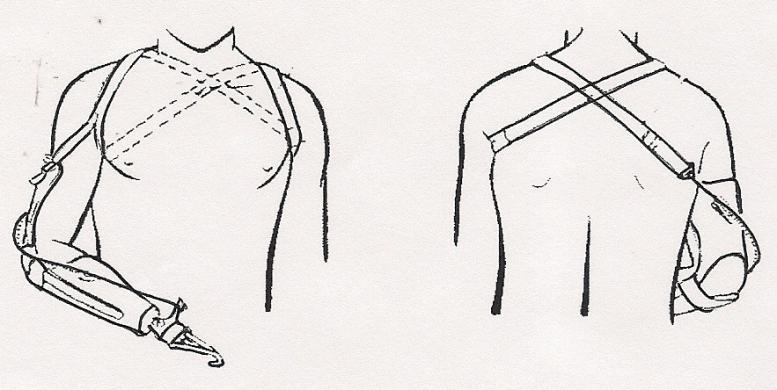
\includegraphics[width=0.62\textwidth,height=\textheight]{img/image_1.jpg}
\caption{Een body-powered prothese met harnas\label{fig:harnas}}
\end{figure}

Ook is de hand aan te sturen via de elektrische signalen uit het brein.
Dit noemt men een neuroprothese. Hier moet de gebruiker mee leren
werken. Ook moet de microcontroller van de hand leren welke acties bij
welke inputs horen. De werking hiervan is omschreven in
\xrefname{Fig.}\cref{fig:leren}.

\begin{figure}
\centering
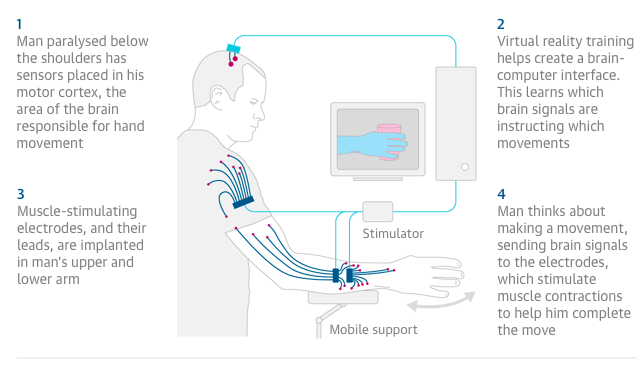
\includegraphics[width=0.62\textwidth,height=\textheight]{img/image_2.png}
\caption{Leren een neuroprothese te gebruiken\label{fig:leren}}
\end{figure}

De derde vorm van het aansturen van een handprothese is via de
armspieren. Deze protheses worden \emph{Myoelectric Controlled
Prostheses} genoemd. Deze protheses meten elektromyografische (EMG)
signalen vanuit de bovenarm. Hier lopen spieren die eigenlijk de hand
aan zouden moeten sturen. De buigspieren, waar de sensoren worden
geplaatst, zitten voornamelijk aan de anteriore\footnote{Vooraanzicht
  lichaam} kant van de arm, met hun antagonisten aan de
posteriore\footnote{Achteraanzicht lichaam} kant van de arm, Taylor
(1999). Deze spieren zijn verlengden van de hand en vingers en lopen als
lange, dunne stroken door de arm. Als hier sensoren op worden geplaatst,
zijn de elektrische signalen die deze spieren afgeven te meten. Als de
signalen versterkt worden, kan de microcontroller het versterkte signaal
gebruiken om de vingers op juiste wijze aan te sturen.

\hypertarget{overige-protheses}{%
\subsubsection*{Overige protheses}\label{overige-protheses}}
\addcontentsline{toc}{subsubsection}{Overige protheses}

Onder overige protheses vallen gehoorprotheses, oogprotheses en
tandprotheses. Deze protheses zijn meestal niet ter vervanging van het
desbetreffende lichaamsdeel, maar omdat dit beschadigd is. Een
gehoorapparaat versterkt de geluidsimpulsen waardoor iemand met een
gehoorbeschadiging toch goed kan horen. Een bril breekt het licht op een
bepaalde manier waarop je toch goed kan zien en een kunstgebit wordt
over je tandvlees of resterende tanden geplaatst waardoor ze eruit zien
als nieuw en het eten en spreken weer een stuk beter gaat. Onder overige
protheses valt ook een borstprothese. De borstprothese wordt ingezet als
iemand als gevolg van bijvoorbeeld borstkanker, haar borst heeft moeten
laten amputeren. Deze protheses bestaan voor het merendeel uit
siliconen. Verschillende borstprotheses zijn benoemd in Danhof (z.d.).
